\section{Esercitazione 3}

Spesso ci sono situazioni in cui guardando certe proprietà del problema numerico da risolvere, si possono trovare degli accorgimenti che risultano avere un impatto non trascurabile sul costo computazionale dell'algoritmo di calcolo. Vediamo di seguito un paio di esempi di questo tipo:

\subsection{Prodotto matrice-vettore}

Supponiamo che sia necessario compiere il prodotto matrice-vettore $A*b$,  in cui la matrice ``A'', di dimensione n x n, è un campionamento della funzione:

\begin{center}  

$f(x,y) = cos(x)*cos(y)$

\end{center}

in una griglia cartesiana di punti nell'intervallo $[0, pi] x [0, pi]$, e ``b'' è un vettore colonna di lunghezza n. Scelti:

\begin{itemize}
\item Un vettore riga di coordinate ``x'' avente n elementi scelti nell'intervallo $[0, pi]$,  e calcolato il vettore ``vx'' tale che  $vx(i) = cos(x(i))$;
\item Un vettore riga di coordinate ``y'' avente n elementi scelti nell'intervallo $[0, pi]$,  e calcolato il vettore ``vy'' tale che  $vy(i) = cos(y(i))$;
\end{itemize}

allora la matrice ``A'' può essere espressa nella forma:

\begin{center}
$A  =  vx' * vy$
\end{center}

dove l'apice significa ``trasposto''.  In generale, essendo A una matrice densa, il prodotto $A*b$ per un generico vettore ``b'' ha un costo dell'ordine di  $O(n^2)$. 

Se, però, utilizziamo l'espressione con cui viene costruita ``A'' ed invertiamo la precedenza nei calcoli:

\begin{center}
$vx' * (vy * b)$
\end{center}

otteniamo una complessità dell'ordine di $O(n)$.
\newline

\textbf{Esercizio}: costruire un programma Matlab/Octave che esegua il prodotto matrice-vettore $A*b$ nelle due modalità qui prospettate e verifichi automaticamente che il risultato del prodotto nei due casi è il medesimo. Inoltre, verificare sperimentalmente, per alcuni valori di n, se l'andamento dei tempi di esecuzione segue l'andamento della complessità qui prospettato e costuire un grafico $(n, tempi)$.

\lstinputlisting[style=customat, caption=Prodotto matrice-vettore]{../Esercitazione3/esercizio1.m}

\begin{figure}[H]
\centering
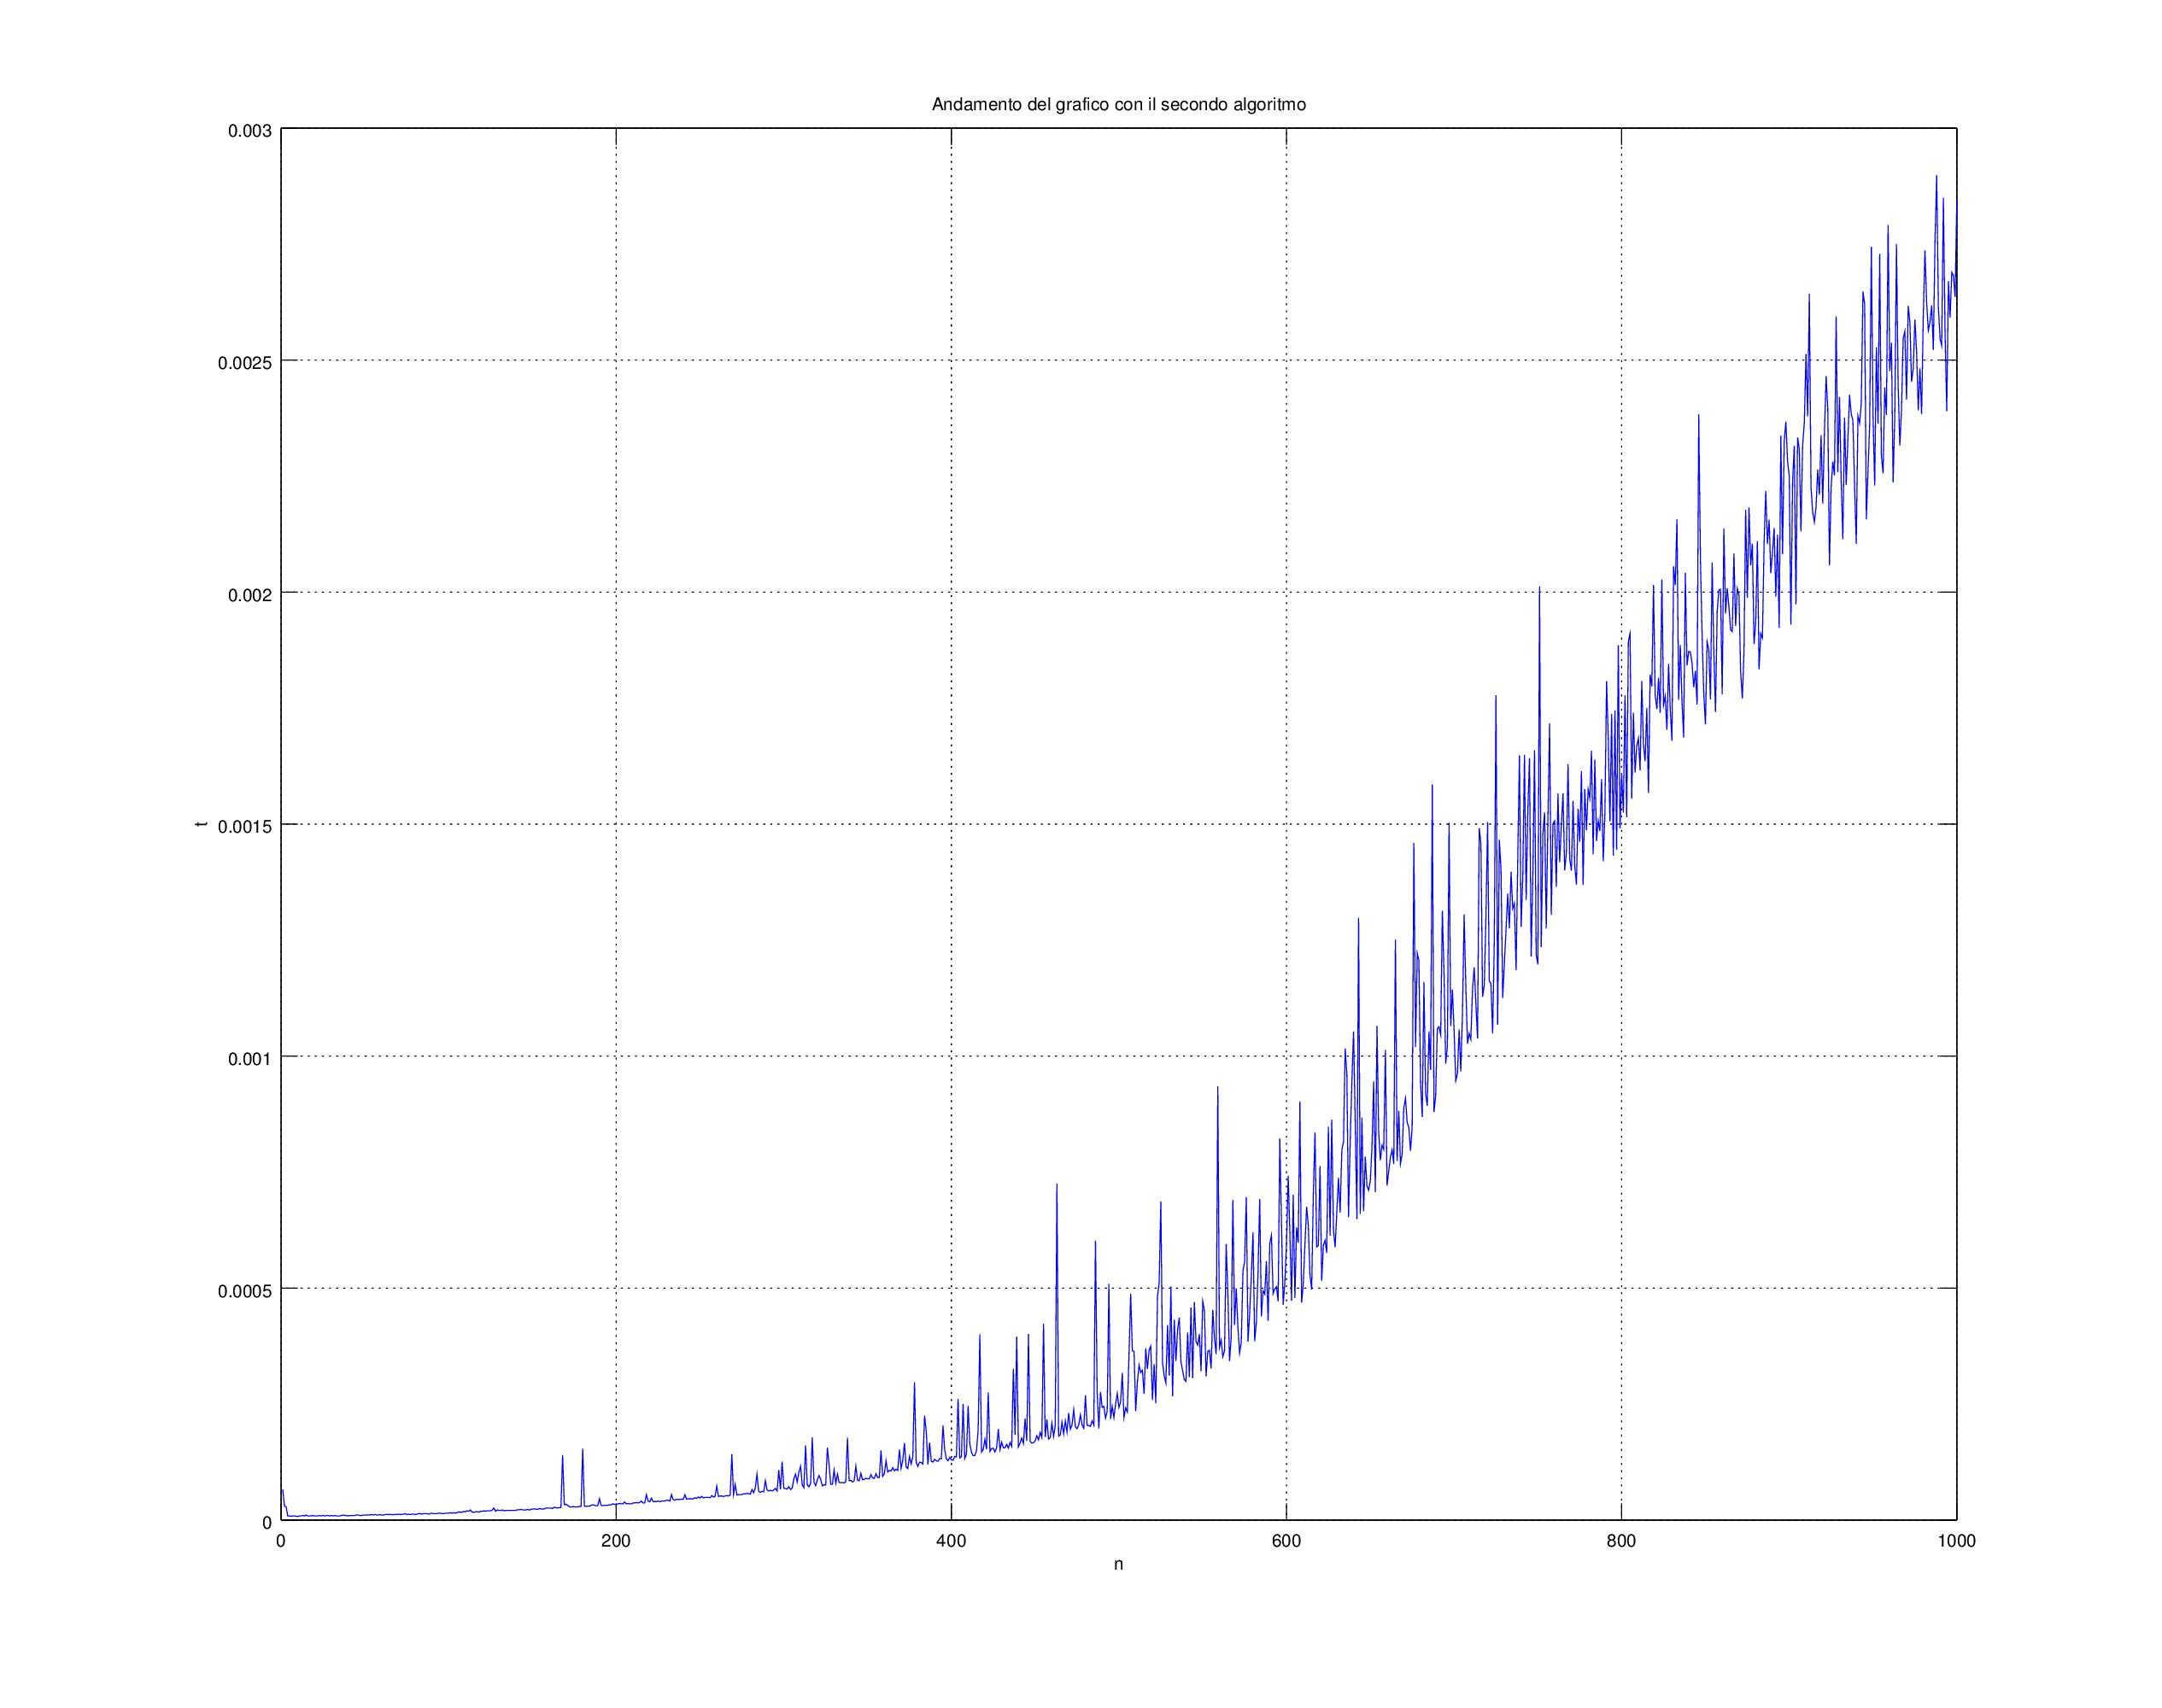
\includegraphics[width=100mm]{../Esercitazione3/images/esercizio1a.jpg}
\caption{Andamento dei tempi nel caso 1}
\label{overflow}
\end{figure}

\begin{figure}[H]
\centering
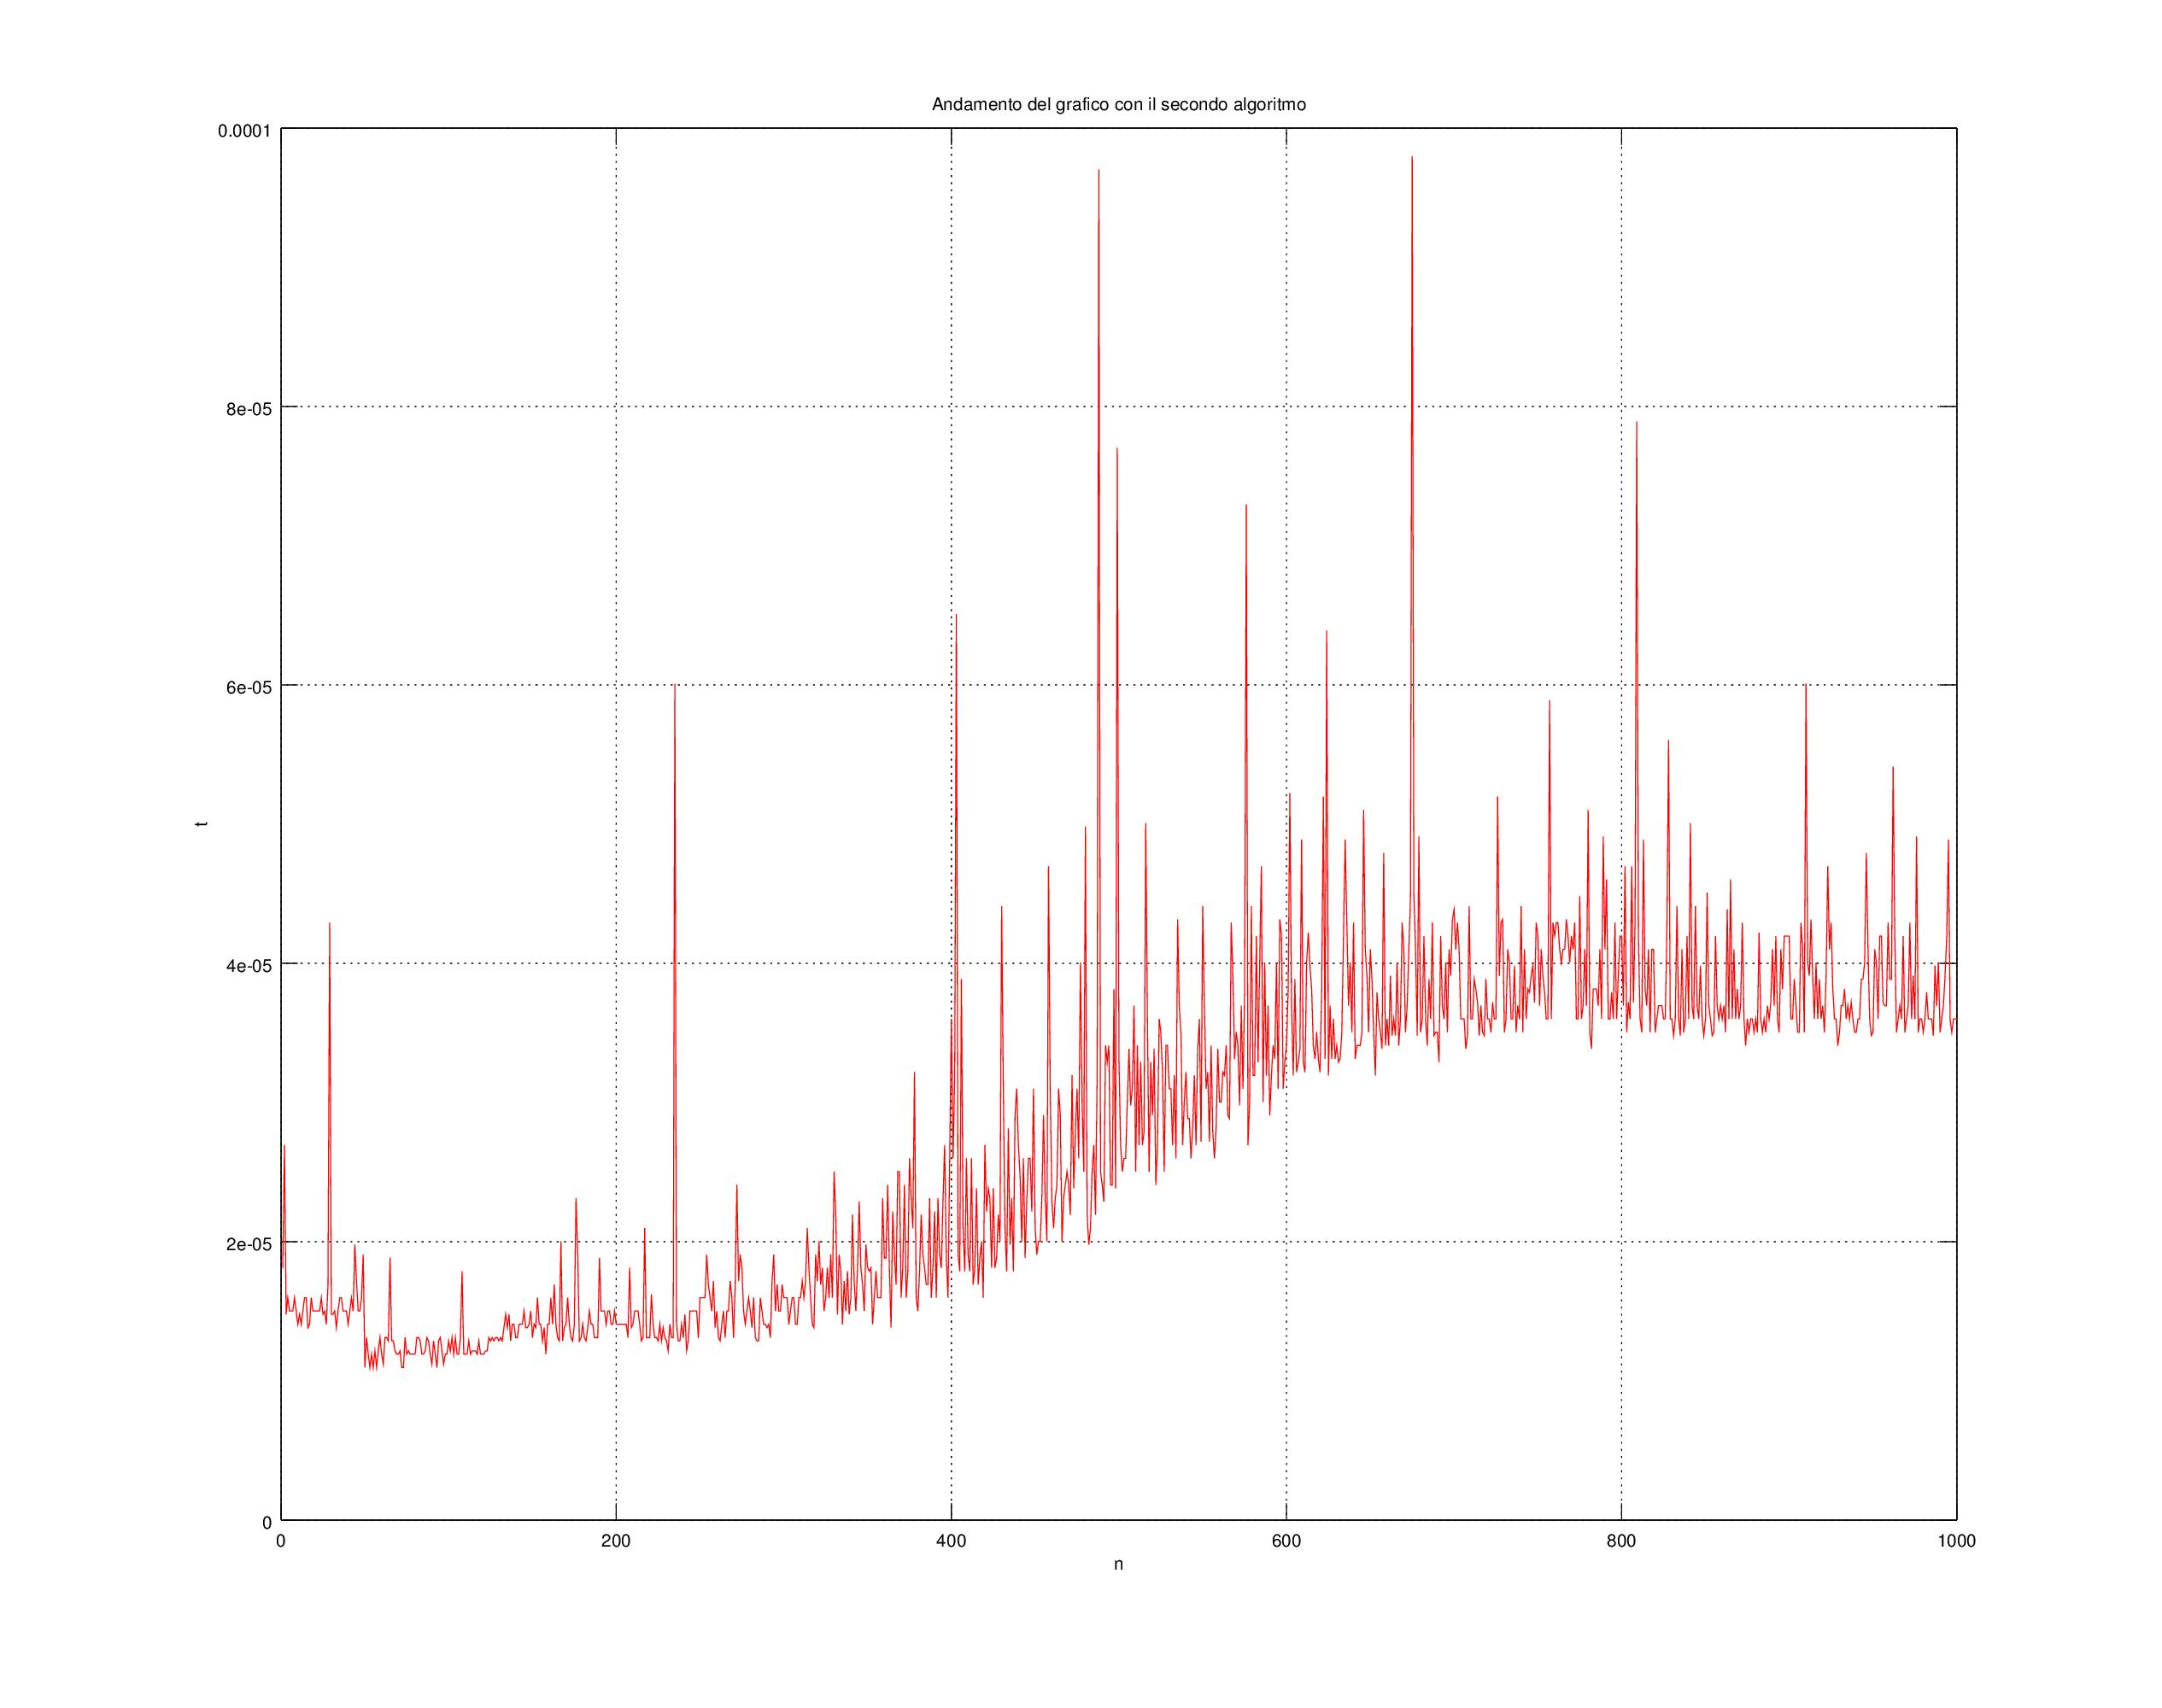
\includegraphics[width=100mm]{../Esercitazione3/images/esercizio1b.jpg}
\caption{Andamento dei tempi nel caso 2}
\label{overflow}
\end{figure}

\begin{figure}[H]
\centering
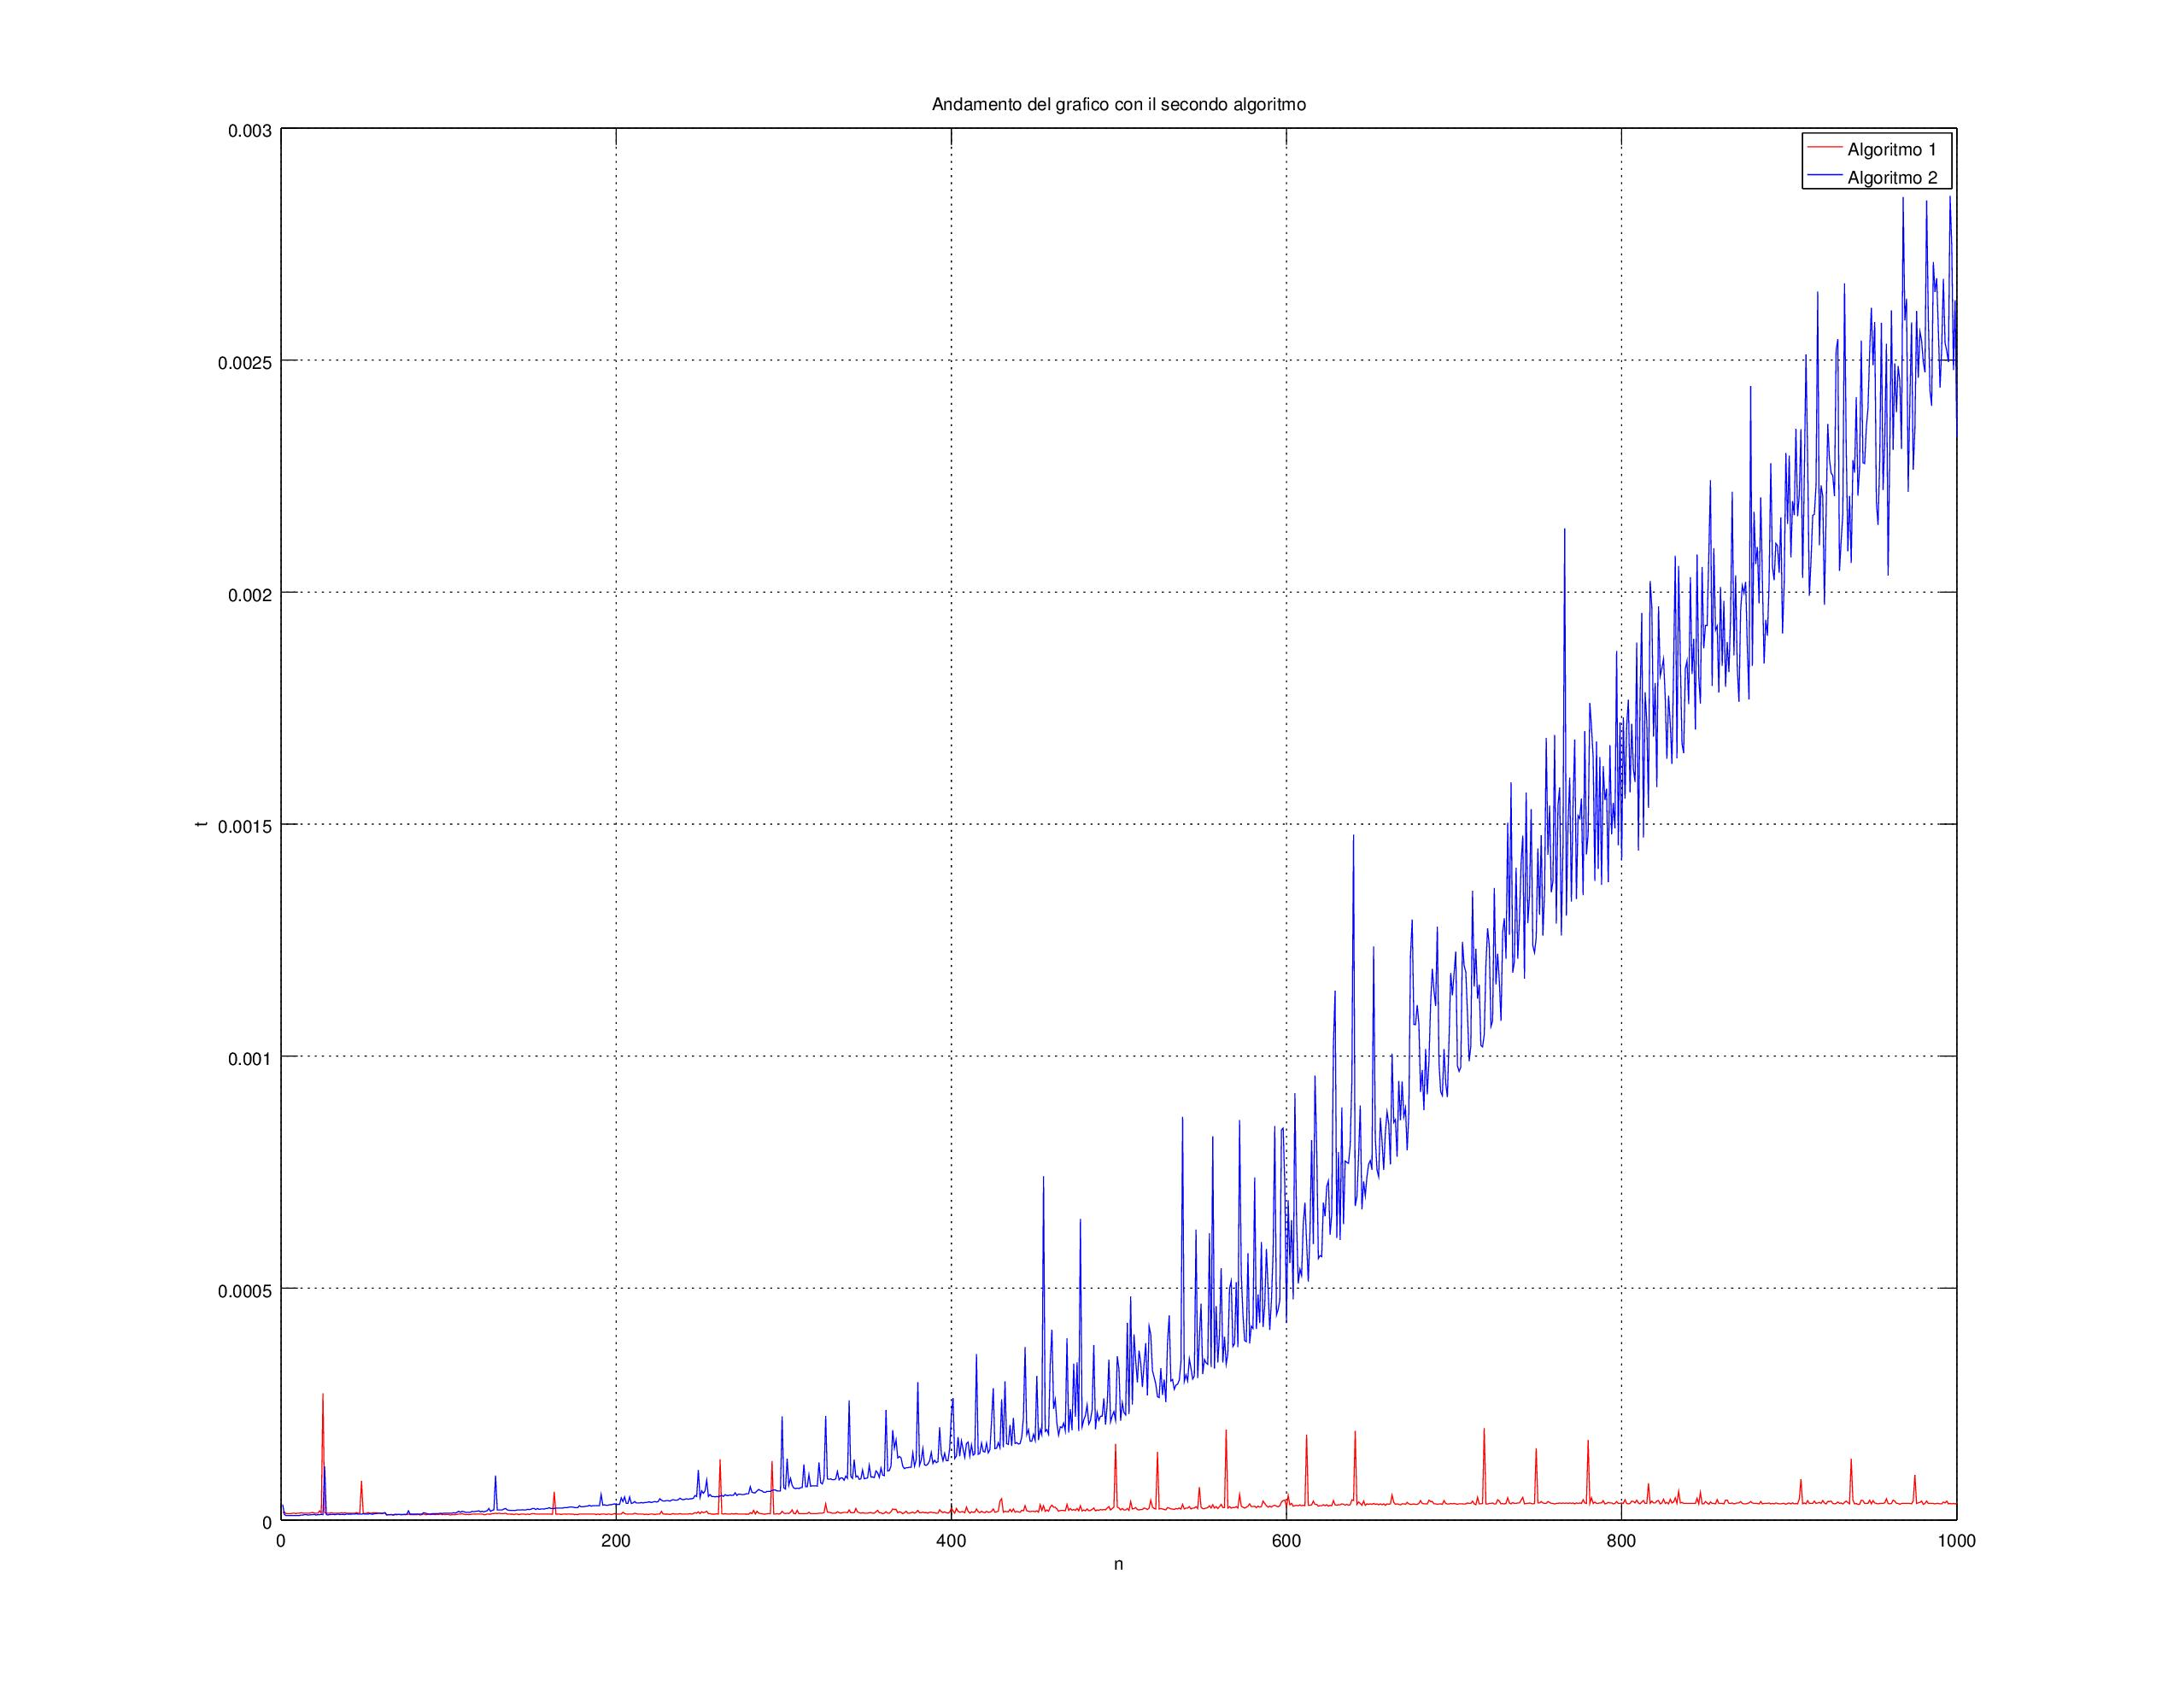
\includegraphics[width=100mm]{../Esercitazione3/images/esercizio1c.jpg}
\caption{Confronto degli andamenti dei due algoritmi}
\label{overflow}
\end{figure}

\subsection{Potenze di matrici}

Per calcolare la potenza q-esima, $q \geq 1$, di una matrice ``A'', si può pensare di moltiplicare ``A'' q-1 volte per se stessa.

In modo più efficiente, possiamo esprimere ``q'' in base-2 (cioè in formato binario), calcolarci i termini $A^{(2^{i})}$,  $i =  1,...,\log{2(q)}-1 = \log{q}/\log{2} -1$ mediante la:

\begin{center}

$A^{(2^i)}  =  A^{(2^{(i-1)})}  *  A^{(2^{(i-1)})}$

\end{center}

e sfruttare il fatto che:

\begin{center}
$A^{(c1 + c2 + c3)}  =  A^{c1}  *  A^{c2}  *  A^{c3}$
\end{center}

\textbf{Esercizio}:  costruire un programma Matlab/Octave che, data una generica matrice ``A'' ed assegnato un valore di ``q'', esegua il calcolo di $A^q$  nelle due modalità qui esposte e verifichi automaticamente che il risultato nei due casi è il medesimo. Inoltre, valutare dal programma qual'è la complessità dei due algoritmi e verificare sperimentalmente, con una matrice ``A'' a scelta e valori di $q = 4,5,...15$ ,  se l'andamento dei tempi di esecuzione segue l'andamento della complessità atteso. Costuire un grafico $(n, tempi)$.

\lstinputlisting[style=customat, caption=Potenze di matrici]{../Esercitazione3/esercizio2.m}